\chapter{Introduction}
\label{sec:introduction}
This chapter will introduce the subject of road and lane detection, and mixed cirticality to the reader. The problems that exist in the field and what the purpose of this degree project is.


\section{Background}
There is a global trend to make vehicles more autonomous to reduce human error and workload. Most modern vehicles include safety-critical systems where a failure can cause great damage to both humans and the environment. When the implementation is a safety-critical system it is important to be aware of the risks that are present and how to cope with them. One other increasingly important trend in the design of real-time and embedded systems is the integration of components with different criticality onto the same hardware platform \cite{burns2013mixed}.\\

The $EMC^2$ project \cite{eu} is an initiative to drive the development of "Embedded Multi-Core systems for Mixed Criticality applications in dynamic and changeable real-time environments". One focus of the project is on automotive applications for example: "Advanced Driver Assistance Systems" (ADAS). ADAS are systems designed to help the driver and to increase the safety when driving. One example is the lane detection system to help keep the car within its lanes \cite{BarHillel2014}. What differs mixed criticality systems from regular systems is that two components with different criticality are run on the same hardware platform. One example could be to run the ADAS and the infotainment system of the vehicle on the same electric control unit (ECU).\\

"Road vehicles -functional safety", ISO 26262 is an international standard for the automotive industry regarding the electronic systems of the vehicles. ISO 26262 defines four automotive safety integrity levels, ASIL A, B, C and D. ASIL A has the lowest integrity requirements and ASIL D has the highest. The problem when implementing two applications of different criticality on the same platform is that both applications need to be certified for the level of the applications with the highest safety requirements. This means that in the case of integrating the ADAS and the infotainment system on the same hardware platform then one would need to certify the infotainment to ASIL D, which is a very tedious and thus expensive task.\\

If it would be possible to isolate the two applications using a technique called virtualization, where applications are run on virtual hardware rather than on bare metal. This approach would not require any extra work on certification compared to running the applications on separate ECUs.\\

The work performed in this thesis project aims at implementing a lane detection system for an autonomus vehicle in a mixed criticality platform. 

\section{Problem statement}
Today there is a lot of research on ADAS where everything from "Lane Departure Warning (LDW)" to "Full autonomous driving" is investigated \cite{BarHillel2014}, \cite{Yenikaya:2013:KVR:2522968.2522970}, \cite{mccall2006video}.\\

However, there is a need for research about the integration of safety critical applications and non-safety critical applications on a mixed criticality platform where the two applications are isolated from each other using virtualization. For an example Autosar, which is a partnership for development of software founded by major players in the automotive industry does address mixed criticality systems in the sense that they recognize that the standards must be supported on their platforms \cite{burns2013mixed} \cite{auto}.\\

This thesis will investigate different techniques for road and lane detection and how they can be implemented on the real-time operating system (RTOS) of a Mixed Criticality System. 


\section{Purpose}
The purpose of the literature study is to give insight in the subject and answer the research question:
\begin{enumerate}  
\item How does a modern lane keeping system function, and how do different systems compare to each other? %In order to study the performance two parameters that could be investigated are: computation time and memory footprint.
\end{enumerate}

After the literature study is done the information will be analyzed and conclusions will be drawn and hopefully above research questions can be answered. From that an implementation phase will begin where the lane detection algorithm should be implemented on  Altens mixed criticality platform which consist of two operating systems on a Xilinx Zynq-7000 board. Figure \ref{fig:Software architecture of  Altens mixed criticality platform} shows how the software architecture of Altens mixed criticality platform is set up. Arm Trustzone is a hardware isolation which does not allow non-secure software from the Linux OS to access secure memory resources which are available for the RTOS. This guarantees that Linux can not interfere with the RTOS called FMP \cite{zaki2016}. SafeG is a hypervisor which decides which operating system should run and when. SHAPE is a cloud for communication between different nodes. Currently SHAPE only works for the Linux OS.


\begin{figure}[H]
  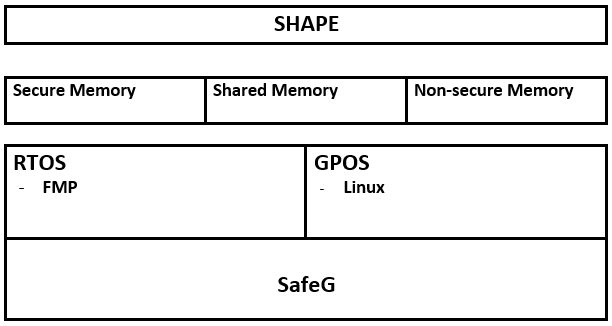
\includegraphics[width=\textwidth]{./img/architecture.png}
  \centering
  \caption{Software architecture of Altens mixed criticality platform}
  \label{fig:Software architecture of Altens mixed criticality platform}
\end{figure}

The goal of the implementation phase is to evaluate how well a practical implementation of lane detection system can perform on a mixed criticality platform. Questions to be answered after the implementation:

\begin{enumerate}  
\item How can we guarantee the performance of the lane detection system?
\item How does the speed of the convoy affect the performance of the lane detection system?
\end{enumerate}

\section{Goals}
In this project there are five master thesis students working together on the same demonstator. This means that there are both individual goals and team goal which do not necessarily align with each other.

\subsection{Team goal}
The team goal is to develop a demonstrator which consists of two small RC-vehicles that are supposed to group into a vehicle convoy where the first vehicle follows a path marked on the ground and the other vehicle follows the first to demonstrate platoon driving.

\subsection{Individual goal}
The individual goal and expected outcome from this thesis is a study of existing road and lane detecting systems. Then comparing different systems to determine which is suitable for implementation in the safety critical system that the group is developing. The last part of the project is to implement the lane keeping algorithm on the RTOS of the mixed criticality system to demonstrate the functionality.

\section{Use case}
This thesis project is part of a larger project conducted by Alten which aims at developing a complete prototype of an intelligent transport system (ITS). In this ITS there will be two vehicles showing the concept of vehicle platooning. The vehicles will be fully autonomous and connected to the infratructure. The project is part of a large EU-project called Safecop which stands for Safe Cooperating Cyber-Physical Systems using Wireless Communication. By using wireless communication one can send commands to the vehicles in the platoon. For example if the conditions are satisfiened, e. g. good connection the ITS can send a command to the vehicle to engage in platoon mode. When they are in platoon mode and one vehicle detects slippery road surface, it can communicate it to the rest of the platoon and the distance between the vehicles can be increased to some predefined safety distance.\\

The vehicles main computing board will contain components of different criticality which means that it is a mixed-criticality system. In a mixed criticality system it is important that the non-safety critical components can not in any way interfere with the safety critical components.\\


This thesis project focuses on the perception problem and the lateral control of the vehicles. The goal is to develop a system that can keep the vehicles within the lane boundaries while keeping satisfactory speed forward. The investigation will be of experimental nature and an evaluation if this platform is appropriate for future use in similar applications will be carried out.


%In the Safecop project description there is mentioned "The US National Highway Traffic Safety Administration (NHTSA) has estimated that “V2V safety applications have the potential to address approximately 80\% of crashes for unimpaired drivers”." The idea is to implement obstacle detection on the road and send out a warning to other vehicles in the platoon or close surrounding.



\section{Delimitations}
The thesis is produced at Alten. Constrained to the Xilinx Zynq-7000 \footnote{https://www.xilinx.com/products/silicon-devices/soc/zynq-7000.html}. The scope of this work extends to investigating lane detection and platoon driving for small vehicles operating in a constructed environment. The results will to some extent depend on the platform that the use case is built upon. In the case of objects on the track some collision avoidance system will be developed and will initially only consist of an emergency break of the vehicle.

\section{Method description}
This degree project will comply with the applied research methodology where information is gathered from accepted and well-known sources and applied to solve specific problems \cite{haakansson2013portal}. To gain knowledge in the field of lane detection systems a literature study will be performed which will guide the development direction of the project.\\

According to Håkansson \cite{haakansson2013portal} an experimental research method is often used and well suited when investigating systems performance. In this degree project the data will be measured and results evaulated on the developed demonstrator.


\section{Ethical considerations and sustainablility}
The work performed in this thesis project is carried out in an as ethical and sustainable way as possible. As always when dealing with automation, it can be important to consider how the system will be used and how the people involved will be affected. One big concern when dealing with automated vehicles is how the decisions are made in situations where accidents occur. In fact there will not even be accidents, but rather decisions made by the computer in the car that led to the situations. The era of automated vehicles will also introduce completely new security threats as the computers in the vehicles can be hacked and overtaken which can lead to injuries and death. Only when the system has been confirmed as safe and secure it can be deployed to real production vehicles.